\chapter{Explain Ridership at Station Level}
% \markright{CHAPTER 2}
%
\section{Introduction}
% \indent % 强制缩进,但 \indent 命令与正文之间需要有一个空行

% brief introduction
Traffic demand forecasting is always an important part of urban planning also urban management, especially in terms of TOD development. To date, most of the studies on predicting rail transit ridership are conducted using the samples of large-scale cities where commonly have a large rail transit system with hundreds of stations. As to medium-sized cities, however, there is also the necessity for traffic demand forecasting. 

% locating this study. brief review
% 说明该类研究多是针对于大城市轨道交通,但中型城市也存在这样的需求。问题在于样本量不足。
In many developed countries like Japan, as the increasingly serious problems of weakness in population growth, adding to the tendency of using private transport in the local central city, operators of public transport, especially urban rail transit, are now facing financial pressure due to the huge operating costs. How to increase the use of public transportation has become an important issue for the government of the local central city in Japan. With the main purpose of turning around the bad financial situation, some efforts already have been made to attract public transit use \cite{takashi2015study}, nevertheless, still far from adequate, particularly for the medium-sized cities. A further and clearer understanding of how various factors affect the ridership is necessary for the policymaker.


% 说明本文要提出一个筛选指标的方法
Using the case of Fukuoka, which is a typical medium-sized local central city in Japan, as the research object, this study can be viewed as an extension of existing station-level ridership model relative to small sample cases. Different from the case with hundreds of samples, a small sample case with dozens of stations has a higher risk of both type I and type II errors in statistic when identifying the valid variables that should be put into the regression model. For this problem, the aim of this study can be stated as: exploring and explaining the factors influencing subway ridership using the small sample case. The main work includes 3 aspects: a. to build the index framework based on prior study; b. to identify the valid indexes that do affect subway ridership; c. to explain the relationship among variables in generating subway ridership quantitatively.

\section{Review}
% overall
To estimate the relevance of various factors and ridership, the model of linear regression is a widely adopted one \cite{cervero1997travel,chakraborty2013land}. However, due to the insufficient consideration of heteroscedasticity and spatial autocorrelation, the result of regression often leads to large standard errors or low level of significance. Thus, linear regression model is not available to all the stations with different characteristics. To improve the generality of the model, the extension such as Geographically Weighted Regression (abbreviated as GWR), Weighted Least Squares Regression (abbreviated as WLS) and Poisson Regression etc. have been successively introduced into the issue of direct ridership model. 

% heteroscedasticity
Chu and Choi et al. estimated the ridership of bus using the model of Poisson Regression \cite{choi2012analysis,chu2004ridership}. The problems occurred in ordinary linear regression such as the contravention between fact and estimated coefficients, and the low level of significance was well addressed. Therefore, both generality and explanatory ability in the regression model were enhanced. Some studies have achieved a high coefficient of determination at the first stage with the ordinary least square model (abbreviated as OLS), however, the result showed a significant heteroscedasticity and a non-random distribution of estimated residual \cite{kuby2004factors}. To deal with this deviation at the second stage, the WLS model was brought in to eliminate heteroscedasticity, in which the data points were weighted using the standard error. The result showed that WLS was effective in eliminating heteroscedasticity and improving the explanatory ability of the model.

%  spatial autocorrelation
The data points in OLS are regarded to be independent of each other, however, each data point has different geographical location in the issue of direct ridership model, the observed values are not considered to be independent of each other in terms of the fact that they are distributed continuously in space. For one data point in regression, the observed value is related to the data point nearby in geographical location, and the regression parameters in different geographical locations usually have different performances in their characteristics \cite{brunsdon1996geographically}. For the problems of spatial autocorrelation and spatial heterogeneity, Cardozo made a comparison of OLS and GWR with the same regression parameters, the result showed that the coefficient of determination had a significant improvement and the standard errors turned to be less in GWR \cite{cardozo2012application}. On the basis of common GWR, Jun and Zhao introduced Mixed Geographically Weighted Regression (abbreviated as MGWR) to this issue in the consideration of that some regression parameters did not have special autocorrelation \cite{jun2015land,zhao2005transit}. They set part of the parameters as global independent variables, and the others as spatially autocorrelated variables, to make model closer to fact.

% summary for review
Although existing studies have done a lot on the issue of direct ridership model, there is still some insufficiency in each study due to the limitation of study case and data source, especially for small sample case. For the selection and construction of factors, the simple and direct indicators such as population, employment etc. are roughly the same with those in the existing studies. But the definition of indicators obtained by secondary calculating such as land use diversity, bus service etc. are not the same, and the effects of such factors have been neither well verified nor widely accepted. For the model, most of the coefficient of determination in OLS were not very ideal (less than 0.7), there was still more than 30\% of the change in ridership not being explained by the model \cite{gutierrez2011transit,jun2015land}. Additionally, even though some of the studies have obtained the high coefficient of determination exactly, there was still another problem that one factor had too strong effect while the rest of the factors had very little influence on the ridership.

% research questions
This study will focus on the small sample case and try to address some of the shortcomings stated above. The main work of this study can be divided into 3 parts. 1) Build the index framework based on the previous studies, and proposes new indicators to help describe the variation in the subway ridership of Fukuoka. 2) Optimize the procedure of identifying a valid explanatory variable, thereby making it applicable for small sample cases. 3) Improve the accuracy in the estimation of the regression model in the terms of small sample cases.

\section{Data}
\subsection{Case introduction}
%
This study focuses on 35 subway stations in Fukuoka City (the sixth largest city in Japan) which has the largest population in Kyushu Island of Japan (more than 1.5 million). Figure \ref{fig:chp2:ResearchArea} is the research area and the distribution of subway stations. Until now Fukuoka has three operating subway lines (The first line was operated since 1981, the second line was operated in 1993 and the latest third line began in 2005), and has a total of 29.8 kilometers operating mileage, some details of the three lines are shown in Table \ref{tab:chp2:DetailsSubway} Details for the three subway lines in Fukuoka. The transport system carries a daily average of more than 0.4 million passengers by 2015 that accounting for more than 20\% in total motorized travel(Ministry of Land, Infrastructure n.d.). Although the subway system of Fukuoka is not a large-scale one, it plays a crucial role in public transportation in terms of the city scale and population.

% Figure 1
\begin{figure}[htbp]
	\centering
	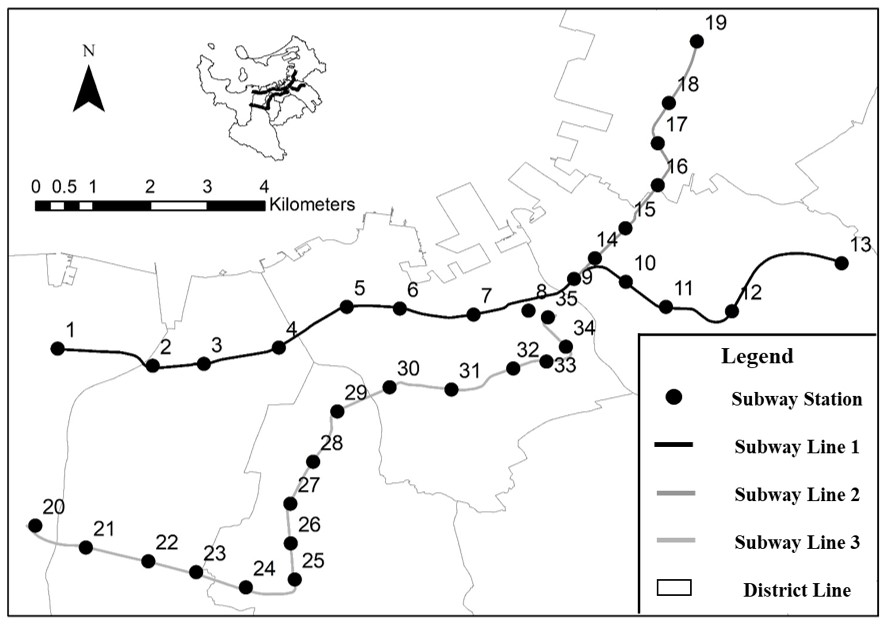
\includegraphics[width=\linewidth]{chp2ResearchArea}
	\caption{Research area and the distribution of subway stations}
	\label{fig:chp2:ResearchArea}
	\small
	\renewcommand{\arraystretch}{1.25} % 重设表间距
\end{figure}

% Table 2
\begin{table}[htbp]
	\centering
	\caption{Details for the three subway lines in Fukuoka}
	\label{tab:chp2:DetailsSubway}%
	\small
	\renewcommand{\arraystretch}{1.25} % 重设表间距
	% 控制表的行间距
	% \renewcommand{\arraystretch}{1}
	% \begin{tabular}[option]{layout} option两个可选,t:按表格顶部对齐,顶部为表格第一行或表线;b:按表格底部对齐,底部是表格第一行或表线
	% \begin{array} 按数学模式制表,可以控制显示的小数点位数等
	\begin{tabular}{cccc}
		\Xhline{1.5pt} % 依赖于 makecell 包
		\diagbox[height=3em]{Item}{Lines} & Line 1 & Line 2 & Line 3\\ % 表头
		\midrule % 依赖于 booktabs 包
		
		% 表内容
		\multicolumn{1}{c}{Total Stations}
		& 13 & 7 & 16\\
		\multicolumn{1}{c}{Operating Distance}
		& 13.1km & 4.7km & 12.0km \\
		\multicolumn{1}{c}{Transfer Station}
		& 5 & 2 & 2\\
		\Xhline{1.5pt}
	\end{tabular}
\end{table}

%
Most of the data used in this study is open source, which can be freely downloaded or bought from the government official website. The data of 2010 year is used as a reference. All the resource of data used in the study is listed below.

%
\begin{itemize}
	\item Subway Ridership
	\item Basic Survey of City Planning
	\item Census
	\item Digital Map (Basic Geospatial Information)
	\item National Land Numerical Information
\end{itemize}

%
\subsection{Catchment area of stations}
%
At present, in the United States, a half-mile-radius (800 m) circle has become the practical standard for rail-transit catchment areas based on TODs \cite{guerra2013half}. The distance of 800m corresponds to the distance people can walk in 10 minutes at the speed of 4.8 km/h. A Japanese case study also supported this 800m catchment area for TOD by using the survey data of $<$2010 big city traffic census metropolitan area report$>$ \cite{tadakatsu2015empirical}. Based on the report of basic survey along the subway third line in Fukuoka, more than 70\% of the passengers choose to walk to the station, about 16\% choose bicycles, the total percentage of non-motorized trip accessing to station accounted for about 90\%. It can be considered that an 800m catchment area covered most of the subway passengers in Fukuoka. On the base of existing literature and the current situation of Fukuoka, the distance threshold of 800m is adopted in this study. All the data based on geographical information will be covered by the 800m PCA using the areal interpolation method.

%
\subsection{Index framework}
%
In this study, the average daily ridership of each subway station is used as the dependent variable. There are 16 variables from the three categories being adopted as candidate independent factors (as shown in Table \ref{tab:chp2:StatisticalDescription}). Some of these variables have already been estimated many times in previous studies, however, there are still some indicators, which may help explain the variation of ridership, ignored in the previous studies. Besides, there is another problem that should be dealt with, the more comprehensive the index framework is, the problem of multicollinearity will occur more easily. For this problem, the candidate variables should be identified and selected by interpret ability in the next stage.

% Table 3
\begin{sidewaystable}[htbp] % sidewaystable 表格横置,依赖于 rotating 包
	\centering
	\caption{Statistical description of candidate independent variables}
	\label{tab:chp2:StatisticalDescription} % \label 一定要在 \caption 之后,否则引用编号会很奇怪
	\small
	\renewcommand{\arraystretch}{1.25} % 重设表间距
	
	% 指定每列宽度
	% tabular 的对齐方式有clrp,c剧中,l居左,r居右,p指定宽度自动换行
	\begin{tabular}{clllrrr}
		\Xhline{1.5pt}
		
		\multicolumn{1}{c}{Category} & % 制作表第一行,用 \multicolumn 是为了区别表题一行与数据的格式
		\multicolumn{1}{l}{Variable} &
		\multicolumn{1}{l}{Unit} &
		\multicolumn{1}{l}{Expected sign} &
		\multicolumn{1}{c}{Min Value} &	
		\multicolumn{1}{c}{Max Value} &	
		\multicolumn{1}{c}{Average}\\
		\midrule
		
		% 数据部分
		% 第一大行
		% 合并多行,依赖于 multirow
		\multirow{7}{90pt}{\centering Land use factors} % 7是合并了7行,90pt是单元格宽度
		& Commerce & ha & + & 0.29 & 81.13 & 11.44 \\
		& Office & ha & + & 0.26  & 84.00 & 16.71 \\
		& Residence & ha & + & 11.08 & 106.75 & 52.85 \\
		& Education & ha & + & 0.03 & 30.56 & 5.97 \\
		& Government & ha & + & - & 12.85 & 2.09 \\
		& Transportation Facility & ha & + & 0.02 & 13.28 & 2.12 \\
		& Land use Aggregation & - & + & 0.09 & 0.75 & 0.31 \\
		\cmidrule{2-7} 		% 2到7列添加横线
		
		% 第二大行
		\multirow{5}{90pt}{\centering Transit-related factors}
		& Transfer Station & Dummy & + & 1.00 & 4.00 & 1.34 \\
		& Bicycle Parking & 100 & Unknown & 0.64 & 43.75 & 7.78 \\
		& Bus Capacity & - & Unknown & 3.00 & 260.00 & 58.48 \\
		& Bus Accessibility & - & Unknown & 4.00 & 455.0 & 89.71 \\
		& Road Density & km/km2 & - & 19.10 & 47.90 & 29.90 \\
		\cmidrule{2-7}
		
		% 第三大行
		\multirow{4}{90pt}{\centering Demographic and socioeconomic environment factors} 
		& Population & Person & + & 1.91 & 19.39 & 9.81 \\
		& House Member & Person & - & 1.86 & 2.79 & 2.18 \\
		& Population Job Balance & - & Unknown & 1.27 & 2.61 & 1.80 \\
		& Ratio of Rental House & \% & - & 0.15 & 0.65 & 0.43 \\
		\Xhline{1.5pt}
	\end{tabular}
\end{sidewaystable}

%
\subsubsection{Land use factors}
%
The land and buildings provide people space for living, working and recreating, and people tend to have different travel preferences with different trip purposes. Therefore, the floor area is commonly thought to be the primary factor that can affect ridership. Another compound indicator, land use diversity, is also thought to be an important factor that can influence transit ridership, because people living in the catchment area with higher land use diversity can do most of their daily activities at different types of buildings without taking public transport.

%
The same with previous studies, this study choose several types of land use with higher proportion to assess the indicator of land use diversity, including residential, office, commercial, education. The four main types of land use account for about 90\% of all the floor area in Fukuoka, especially in subway catchment area, reaching more than 95\%. However, different from the general definition of land use diversity, the proportion of land use is not evenly distributed in the case of Fukuoka City. As shown in Table \ref{tab:chp2:LandUse}, obviously, it is significantly different from average distribution, and the proportion varies with the variation of the catchment area. To describe the land use diversity closer to the facts, the referenced balance proportion of land use types is decided by the average proportion of all subway station catchment area (800m pedestrian distance) in Fukuoka.

% Table 4
\begin{table}[htbp]
	\centering
	\caption{Average proportion of each land use type in different PCA}
	\label{tab:chp2:LandUse}%
	\small
	\renewcommand{\arraystretch}{1.25} % 重设表间距
	% 控制表的行间距
	% \renewcommand{\arraystretch}{1}
	% \begin{tabular}[option]{layout} option两个可选,t:按表格顶部对齐,顶部为表格第一行或表线;b:按表格底部对齐,底部是表格第一行或表线
	% \begin{array} 按数学模式制表,可以控制显示的小数点位数等
	\begin{tabular}{ccccc}
		
		\Xhline{1.5pt} % 依赖于 makecell 包
		\diagbox[height=3em]{Range}{Type} & Business & Commerce & Residence & Education\\ % 表头
		\midrule % 依赖于 booktabs 包
		
		% 表内容
		\multicolumn{1}{c}{600 m}
		& 20.8\% & 14.9\% & 55.7\% & 6.0\%\\
		\multicolumn{1}{c}{800 m}
		& 18.8\% & 12.8\% & 59.4\% & 6.7\%\\
		\multicolumn{1}{c}{1000 m}
		& 17.7\% & 11.6\% & 62.0\% & 6.5\%\\
		\multicolumn{1}{c}{City Average}
		& 10.5\% & 7.7\% & 65.2\% & 5.5\%\\
		\Xhline{1.5pt}
	\end{tabular}
	\normalsize
	\begin{description}
		\label{note:tab:chp2:LandUse}
		\item[Note:]
		The value marked with grey is adopted in this study.
	\end{description}
\end{table}

%
In addition, to make indicator more intuitive and simpler, the index of land use diversity is redefined as the aggregation of land use. The Euclidean Metric is used for evaluating the deviation of land use aggregation in each subway station with respect to a reference value. The value of this indicator is arranged from 0 to $\sqrt{2}$, in which the lower value represents a higher level of mixing in land use function, while the higher value means the land use function is more monotonous. This indicator of land use aggregation is defined as Equation \ref{eq:chp2:LanduseAggregation}, it is speculated to have a negative impact on ridership.

% eq 1
\begin{equation}
	G=\sqrt{\sum \left ( A_{i}-P_{i} \right )^2}
	\label{eq:chp2:LanduseAggregation}
\end{equation}
% note for eq 1
\begin{description}
	\item[Where:]
	the $G$ is the indicator for aggregation of land use functions, $P_i$ is the average proportion of $i$ type land use, $i$ represents the type of land use (respectively government, commercial, residence and education), $A_i$ is the proportion of land use type $i$ within catchment area of subway station.
\end{description}

\subsubsection{Transit-related factors}
%
The transit-related factors are thought to affect subway ridership in two opposite ways. Higher accessibility for accessing into the catchment area of subway station means people will have more transportation options to get into the area instead of the subway, such as private cars, bicycle, bus or walking etc. On the other hand, higher accessibility also allows people to arrive station more easily, and then attract passengers to use the subway. Considering different travel modes, accessibility is separated into 3 parts to be interpreted in this study. First is for users of the road network; second is for passengers transferring from the bus; third is for rail transit interchange.

%
Road network is commonly used in previous studies. Users of the road network are not only the vehicle but also non-motorized travelers including bicycle riders and pedestrians. As is known, the higher coverage of road network is thought to have better accessibility for both motor travel and non-motorized travel. Additional, bicycle parking may also be an important factor influencing the accessibility of catchment area for non-motorized travelers. Therefore, the accessibility index for road network is set into the number of bicycle parking and road density in this study.

%
Another accessibility for passengers transferring from the bus is also considered from both positive and negative way. Bus service in catchment area can reflect the connectivity with other regions, by which the potential subway ridership can be shared by bus to some extent. This sharing ridership can be represented by the service capacity of all the bus operating in the same catchment area of the subway station, and the service capacity $(C)$ is expressed by Equation \ref{eq:chp2:BusCapacity} as follow. In contrast, the bus station close to subway can be used as transfer station which can increase the accessibility of subway for people who want to take the subway but living far away from subway station. In this case, the bus station will play a positive effect on ridership of subway. The indicator should represent the accessibility between subway and bus, thus it is defined as the number of bus lines within the catchment area of subway station. The indicator A representing accessibility of bus is defined as Equation \ref{eq:chp2:BusAccessibility} in the below.

% eq 2
\begin{equation}
	C=\sum_{k}^{K}\sum_{r}^{R}f_{r}^{k}
	\label{eq:chp2:BusCapacity}
\end{equation}

% note for eq 2
\begin{description}
	\item[Where:]
	the $K$ is the number of bus stations within catchment area of subway station, $R$ refers to the number of lines in one bus station and $f_r^k$ is the frequency of the $r$th line at the $k$th station.
\end{description}

% eq 3
\begin{equation}
	A=\sum_{k}^{K}R_{k}
	\label{eq:chp2:BusAccessibility}
\end{equation}

% note for eq 3
\begin{description}
	\item[Where:]
	the $K$ is the number of bus stations within catchment area of subway station, $R_k$ is the number of bus lines passing through the $k$th bus station.
\end{description}

%
Because the existing rail transit network is relatively stable and unchanging, the convenience of railway interchange is roughly determined by the characteristic of the subway station. The accessibilities are different in diverse types of station: intermediate, terminal, interchange, intermodal. Terminal station is generally thought to have a larger catchment area since the terminal station is probably the only choice for the people living far away from the station when they want to take the subway. And people can accept spending more time on getting into the terminal station \cite{o1996walking}. Interchange station and intermodal station are attractive for passengers since it can connect to other lines of railway transit or other modes of transportation \cite{kuby2004factors}. To distinguish the difference between different types of stations, the dummy variable for describing the number of railway lines passing through each station is introduced into this study.

%
\subsubsection{Demographic and socioeconomic environment factors}
%
For this group of factors, except for the population and employment factors, age structure and household member are also considered to have effect on travel habit. In addition, the family with more working people tends to generate more travel, therefore the indicator of population-to-employment is also thought to be one of the determinants. The factor of tenant proportion was considered to have negative effect on subway ridership in previous studies. Because renters are commonly commute-oriented, they prefer to live close to where they are working and usually commute by walking.

%
All the 16 candidate indicators are shown in Table \ref{tab:chp2:StatisticalDescription}. According to the previous studies, an expected influence is shown in the column of expected sign. With the consideration of small sample case in this study, the method is divided into two phases, identifying the valid variables and estimating the coefficients.

%
\section{Methods}
%
The exploratory regression tool in ArcGIS is introduced into this study to help to conduct the process of identifying valid variables. As is known, finding a proper OLS model is the main problem in this kind of study, especially when there are lots of candidate explanatory variables being estimated in the regression model. The Exploratory Regression tool provides a reference for choosing a valid combination of explanatory variables. It is a data mining tool that will try all possible combinations of explanatory variables to see which model can pass the necessary OLS diagnostics. This study proposes a two-step procedure to explore the final model with an optimal combination of explanatory indicators, rather than selecting the best one from all possible combinations. The first step is selecting the variables having effectiveness in explaining the subway ridership, and the second step is choosing the best combination of the valid variables in the final indicators.

%
GWR is a spatial regression technique, which is used for dealing with the explanatory variables with spatial dependence. The coefficients of explanatory variables are varied with the spatial location of the data point in GWR, and the closer the distance between a data point and observation point is, the greater weight the data point is. Different from general GWR, the explanatory variables in MGWR can be either spatial dependent or spatial independent. The variables with spatial dependence (called local variable) are the same with that in GWR, varied with spatial location of data points; while the variables without spatial dependence (called global variable) are the same with that in OLS, constant in all data points. Before estimating the MGWR model, it is necessary to determine whether the variable is spatial dependent or not. To prevent this small sample case from becoming data-driven, repeating test is conducted to reduce the probability of occasional mistakes. The local/global variables were determined by the spatial dependency of each exploratory variable, in which the variable with spatial dependency is treated as a local term, otherwise, is treated as a global term.

%
\section{Results}
\subsection{Selection of effective variables}
%
The first stage of selecting effective variables is conducted based on three judgment factors: a. Multicollinearity, which is expressed by the factor of VIF; b. Validity, which is expressed by the number of times that shows statistical importance; c. Stability, which is shown by the percentage of negative and positive effect to the dependent variable (Stage 1 in Table \ref{tab:chp2:ExploratoryRegression}). Generally, the variable is thought to be multicollinearity if the value of VIF factor is more than 7.5, as shown in Table \ref{note:tab:chp2:ExploratoryRegression} there are four variables with higher VIF which are marked by dark color. For the factor of validity, three variables are filtered since they rarely show their statistical significance (less than 10\%). Even though some variables have statistical significances in the regression model, they are still not credible since their performances are not stable in different models (sometimes they are positive for the independent variable but sometimes are not). As shown in the underneath of stage 1 in Table \ref{note:tab:chp2:ExploratoryRegression}, the three variables marked with grey are shown not stable in explaining dependent variable. Therefore, as a result, 10 valid variables of 16 candidate variables are reserved in the first stage.

% Table 5
\begin{sidewaystable}[htbp]
	\centering
	\caption{Results of the exploratory regression}
	\label{tab:chp2:ExploratoryRegression}%
	\small
	\renewcommand{\arraystretch}{1.25} % 重设表间距
	\begin{tabular}{clrrrrrcrrr}
		\Xhline{1.5pt}
		
		% 表题第一行,Stage 1和Stage 2
		\multirow{3}[4]{*}{Variable} & \multirow{3}[4]{*}{Unit} & & \multicolumn{4}{c}{Stage 1} & & \multicolumn{3}{c}{Stage 2} \\
		
		% 表题第二行,Statistical... 和 Test Model
		& & & \multicolumn{4}{c}{Statistical Information} & & \multicolumn{3}{c}{Test Model} \\
		
		% 第一行的下划线
		\cmidrule{4-7} \cmidrule{9-11}
		
		% 表题第三行,VIF, Validity, Stability...
		& & & VIF & Validity & Stability & Times & & B & Sig & VIF \\
		
		% 第二行的下划线
		\cmidrule{1-2}\cmidrule{4-7}\cmidrule{9-11}
		
		% 表的正文上半部分
		Government & ha & & 1.8 & 42.30\% & 100.00\% & 33 & & 490 & 0.02  & 1.36 \\
		Transportation Facility & ha & & 3 & 67.90\% & 100.00\% & 53 & & 1180 & 0 & 2.31 \\
		
		Land use Aggregation & \% & & 2.5 & 50.00\% & 100.00\% & 39 & & 124 & 0.03 & 1.42 \\
		
		Transfer Station & Dummy & & 3 & 34.60\% & 100.00\% & 27 & & 6014.28 & 0 & 2.79 \\
		
		Bicycle Parking & 100 & & 4.5 & 44.90\% & 100.00\% & 35 & & 754 & 0 & 2.6 \\
		
		Bus Capacity & - & & 6.6 & 37.20\% & 96.60\% & 29 & & -68.19 & 0.01 & 3.56 \\
		
		Bus Accessibility & - & & 6.8 & 19.20\% & 100.00\% & 15 & & 49.37 & 0 & 4.71 \\
		
		Job-Resident Balance & \% & & 3 & 37.20\% & 100.00\% & 35 & & -47.08 & 0.05  & 1.94 \\
		
		Tenant Proportion & \% & & 2.2 & 21.80\% & 100.00\% & 29 & & -138.2 & 0.03  & 1.32 \\
		
		Household Members & \% & & 3 & 39.70\% & 100.00\% & 27 & & - & - & - \\
		
		% 第三行下划线
		\cmidrule{1-2}\cmidrule{4-7}\cmidrule{9-11}
		
		% 表的正文下半部分
		Commerce & ha & & \cellcolor[rgb]{ .8,  .8,  .8}8.8 & 32.10\% & 100.00\% & 25 & & &  \\
		
		Office & ha & & \cellcolor[rgb]{ .8,  .8,  .8}10.4 & \cellcolor[rgb]{ .8,  .8,  .8}9.00\% & \cellcolor[rgb]{ .8,  .8,  .8}71.40\% & 7 & & \multicolumn{2}{l}{Residual sum of squares} & 337744990 \\
		
		Residence & ha & & \cellcolor[rgb]{ .8,  .8,  .8}27.5 & 12.80\% & \cellcolor[rgb]{ .8,  .8,  .8}70.00\% & 10 & & \multicolumn{2}{l}{Adjusted R2} & 0.96 \\
		
		Education & ha & & 1.8 & \cellcolor[rgb]{ .8,  .8,  .8}7.70\% & 100.00\% & 6 & & \multicolumn{2}{l}{AICc} & 694.39 \\
		
		Road Density & km/km2 & & 2.3 & \cellcolor[rgb]{ .8,  .8,  .8}1.30\% & 100.00\% & 1 & & \multicolumn{2}{l}{Jarque-Bera test (Sig)} & 0.61 \\
		
		Population & person & & \cellcolor[rgb]{ .8,  .8,  .8}23.9 & 12.80\% & \cellcolor[rgb]{ .8,  .8,  .8}60.00\% & 10 & & \multicolumn{2}{l}{Koenker (BP) test (Sig)} & 0.85 \\
		
		\Xhline{1.5pt}
	\end{tabular}%
	\normalsize
	\begin{description}
		\label{note:tab:chp2:ExploratoryRegression}
		\item[Note:]
		The value marked with grey means it is not valid.
	\end{description}
\end{sidewaystable}%

%
At the second stage, the exploratory regression is conducted again to select an optimal combination of explanatory variables based on a statistical test for regression. As shown in the stage 2 of Table \ref{tab:chp2:ExploratoryRegression}, the variable of household members did not pass the statistical significance test, there are 9 valid variables entering the model at last (at 95\% confidence level). The Jarque–Bera test (Abbreviated as JB test) is not significant in the final model; it indicates that there are no biased standard errors due to heteroscedasticity. The Breusch–Pagan test is not showing statistical significance, it represents that the residuals are not deviating from a normal theoretical distribution. The test of SA is not significant; it means the residuals are not spatial autocorrelated. The optimal combination with 9 explanatory variables will be evaluated by using MGWR in the next part to obtain a better result with fewer residuals.

\subsection{Estimation of MGWR}
%
The MGWR is estimated is estimated by using a fixed Gaussian kernel function,  the optimal bandwidth size is determined by using a “golden-section search” method. As a result, the optimal bandwidth is obtained when its corresponding AICc value gets to the minimum. The variation of AICc at different bandwidths are shown in Figure \ref{fig:chp2:AICcBandwidths}, and the optimal bandwidth is to the lowest AICc of 5.7 km.

% Figure 2
\begin{figure}[htbp]
	\centering
	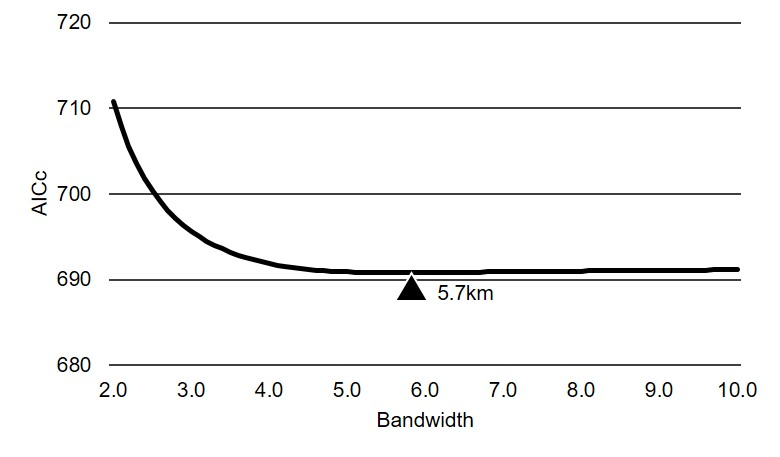
\includegraphics[width=\linewidth]{chp2AICcBandwidths}
	\caption{Variations of AICc at different bandwidths}
	\label{fig:chp2:AICcBandwidths}
\end{figure}

The determination of local or global is processed in two steps: firstly, using Moran’s index to examine if the variable is spatial autocorrelation or not; secondly, re-examining the variable with spatial dependency in terms of the indicator of “DIFF of Criterion” provided by GWR4. The test value describing the spatial relationship is summarized in the left part of Table \ref{tab:chp2:ResultMGWR}. Five variables are found to be spatial autocorrelation; they are transportation warehousing, bus capacity, bus accessibility and the tenant proportion respectively. Thereby in the first step, the other 4 variables are considered as global variables while the 5 variables with spatial dependency are considered as local variables. Nakaya, the author of the GWR4 software suggested in the GWR4 user manual that the assessment of the spatial variability of the $k$th varying coefficient is conducted by comparing the fitted GWR with a model in which only the $k$th coefficient is fixed while the other coefficients vary spatially \cite{nakaya2014gwr4}. If the original model is better than the model with the kth coefficient fixed, that coefficient can be considered as spatial autocorrelation. GWR4 also provides the indicator of model comparison which is “DIFF of Criterion”. The user manual suggests that a positive value of “DIFF of Criterion”, especially greater than or equal to 2, means the local term is better to be assumed as a global one. As shown in the left part of Table \ref{tab:chp2:ResultMGWR}, all the values of indicator “DIFF of Criterion” are no more than 2, which means that all the local terms are adapt to the model. Therefore, all the local variables passed the test in the second step.

% Table 6
\begin{sidewaystable}[htbp]
	\centering
	\caption{Results of MGWR model}
	\label{tab:chp2:ResultMGWR}
	\small
	\renewcommand{\arraystretch}{1.25} % 重设表间距
	
	\begin{tabular}{clrrrrrrrrr}
		\Xhline{1.5pt}
		\multicolumn{1}{c}{\multirow{2}[4]{*}{Variable}} & \multicolumn{6}{c}{Spatial distribution characteristics of final explanatory variables} & & \multicolumn{3}{c}{MGWR model} \\
		
		\cmidrule{2-7}\cmidrule{9-11}
		
		& \multicolumn{1}{p{3em}}{Unit} & \multicolumn{1}{p{4em}}{Moran's Index} & P-Value* & Pattern & Type & \multicolumn{1}{p{4em}}{DIFF of Criterion} & & Coefficient & SE & t \\
		
		\cmidrule{1-7}\cmidrule{9-11}
		
		Government & ha & 0.04 & 0.51 & Random & Global &- & & 490 & 190 & 2.59 \\
		Transportation Facility & ha & 0.29 & 0 & Clustered & Local & -1.95 & & 1020 & 200 & - \\
		Land use Aggregation & \% & -0.01 & 0.84 & Random & Global & - & & 133.84 & 54.06 & 2.48 \\
		Transfer Station & Dummy & 0.13 & 0.12 & Random & Global & - & & 5968.65 & 1198.72 & 4.98 \\
		Bicycle Parking & 100 & -0.12 & 0.36 & Random & Global & - & & 771.7 & 89.8 & 8.59 \\
		Bus Capacity & - & 0.7 & 0 & Clustered & Local & 0.18  & & -55.16 & 5.94  & - \\
		Bus Accessibility & - & 0.45 & 0 &  Clustered & Local & 0.04 & & 48.61 & 2.43 & - \\
		Job-Resident Balance & \% & 0.77 & 0 & Clustered & Local & -0.17 & & -24.11 & 3.64 & - \\
		Tenant Proportion & \% & 0.24 & 0.01 & Clustered & Local & 1.02 & & -103.05 & 7.56 & - \\
		
		\midrule
		
		\multicolumn{5}{l}{\multirow{3}[2]{30em}{\textbf{Note:} Confidence level 95\%. If p-value is less than 0.05, the corresponding variable can be viewed as a local one.}} & \multicolumn{4}{r}{Best bandwidth} & \multicolumn{2}{r}{5.7km} \\
		\multicolumn{5}{l}{} & \multicolumn{4}{r}{AICc} & \multicolumn{2}{r}{690.6} \\
		\multicolumn{5}{l}{} & \multicolumn{4}{r}{Residual sum of squares} & \multicolumn{2}{r}{296311499} \\
		
		\Xhline{1.5pt}
	\end{tabular}%
\end{sidewaystable}%


\subsection{Interpretation of coefficients}
%
The right part of Table \ref{tab:chp2:ResultMGWR} reports the result of MGWR model. The global variables in MGWR model have statistical significance at 95\% confidence level, it means most of the variation in ridership can be explained by the 9 variables in this present model. The signs of all terms for local variables are consistent with that of OLS model in Table \ref{tab:chp2:ExploratoryRegression}, and the values of coefficients in MGWR maintain a high consistency with OLS model. The result shows that there are 3 variables, which are bus capacity, job-resident balance, and tenant proportion, impacting negative effect on ridership, while the others 6 variables play positive effect. The value of the explanatory variable changes by 1 unit, the subway passenger will change the value of the coefficient. It is interesting to note from the coefficient that although the variables of bus capacity and bus accessibility have a strong positive correlation with statistical significance, they perform completely opposite effect on the independent variable. Moreover, comparing with the result of OLS regression, the result of MGWR has an improvement in both adjusted R2 and AICc value, and there is a 12\% decrease in residual.

% Table 7
\begin{table}[htbp]
	\centering
	\caption{Residual spatial autocorrelation of OLS and MGWR}
	\label{tab:chp2:Residual}%
	\small
	\renewcommand{\arraystretch}{1.25} % 重设表间距
	
	\begin{tabular}{crr}
		\Xhline{1.5pt}
		Index & OLS & MGWR \\
		
		\midrule
		Moran’s index & 0.08  & 0.03 \\
		Expected index & -0.03 & -0.03 \\
		Variance & 0.01  & 0.01 \\
		z-score & 1.09  & 0.61 \\
		p-value & 0.27  & 0.54 \\
		
		\Xhline{1.5pt}
	\end{tabular}
\end{table}

%
\subsection{Evaluation of results}
%
As the result from both models, MGWR has a better performance than OLS, in which the residual of MGWR is 12.27\% less than that of OLS. Also, the homogeneity of residual distribution is evaluated by using Moran’s index shown in Table \ref{tab:chp2:Residual}. As can be seen, the Moran’s index in MGWR is closer to expected value than that in OLS. The MGWR model also shows less variance and greater likelihood of random distribution (with lower z-score and higher p-value) than OLS model. The spatial autocorrelation analysis presents that the residual of OLS model is more likely to be aggregative in space.

% Figure 3
\begin{figure}[htbp]
	\centering
	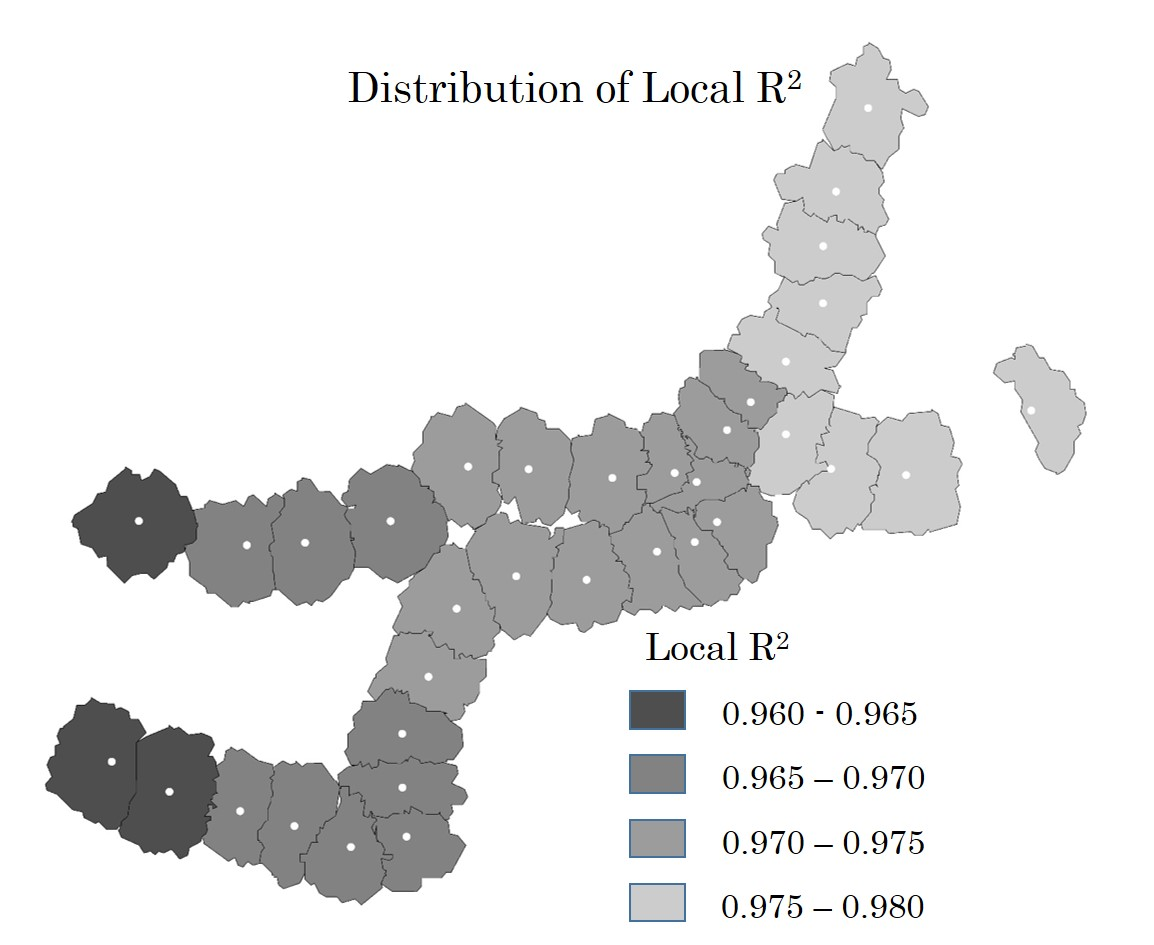
\includegraphics[width=\linewidth]{chp2LocalR}
	\caption{The spatial distribution of local $R^2$}
	\label{fig:chp2:LocalR}
\end{figure}

%
Since the MGWR is a kind of variable coefficient regression model, the coefficients and adjusted R2 of each data point are different depending on the location of the data point, as shown in the Figure \ref{fig:chp2:LocalR}. For the 5 local variables in all 35 data points, the spatial distribution of significance level for the local variables are mapped in Figure \ref{fig:chp2:SignificanceDistribution}. For the variables of building area of transportation, bus capacity, bus accessibility, job-resident balance and tenant proportion, there are 33, 34, 35, 24 and 32 data points having statistical significance at confidence level 95\% respectively. As can be seen, the two indicators for bus proposed in this study have good performance in terms of significance and stability, while the variable of ‘tenant proportion’ does not have a strong stability in explanatory ability. Relatively, the other 4 variables have higher reliability in explaining the variety of ridership.

% Feagure 4

% 多图联排的模板

% 如果使用\usepackage{subfig},可以对每个子图进行交叉引用
% 用法:\subfloat[...]{\label{sub-fig-1}% 为子图加交叉引用,详见该包的说明
% Note: 两个minipage之间不能有空行,否则无法对齐

% \begin{figure}[] 位置参数的说明
% [h]  表示的当前位置(here),也就是说图片排在你设置的当前位置,但是如果这一页的空间不足以放下这个图片,此时图片会转到下一页。
% [t]  顶端(top)。此时系统会将图片放置在页面的顶部。
% [b] 底部. (bottom) 这里是优先将图片放置在底部,也就是页面的底部。
% [p]  这个是将图片设置为浮动状态,也就是可以根据系统排版的,自动放置图片的位置。
% [htbp] 优先放置在最佳位置,然后将其放在顶端最后放在底部,最后设置为浮动状态。
\begin{figure}[htbp]
	% 两列排列,每列占宽0.48
	\begin{minipage}{0.48\linewidth}
		\centering
		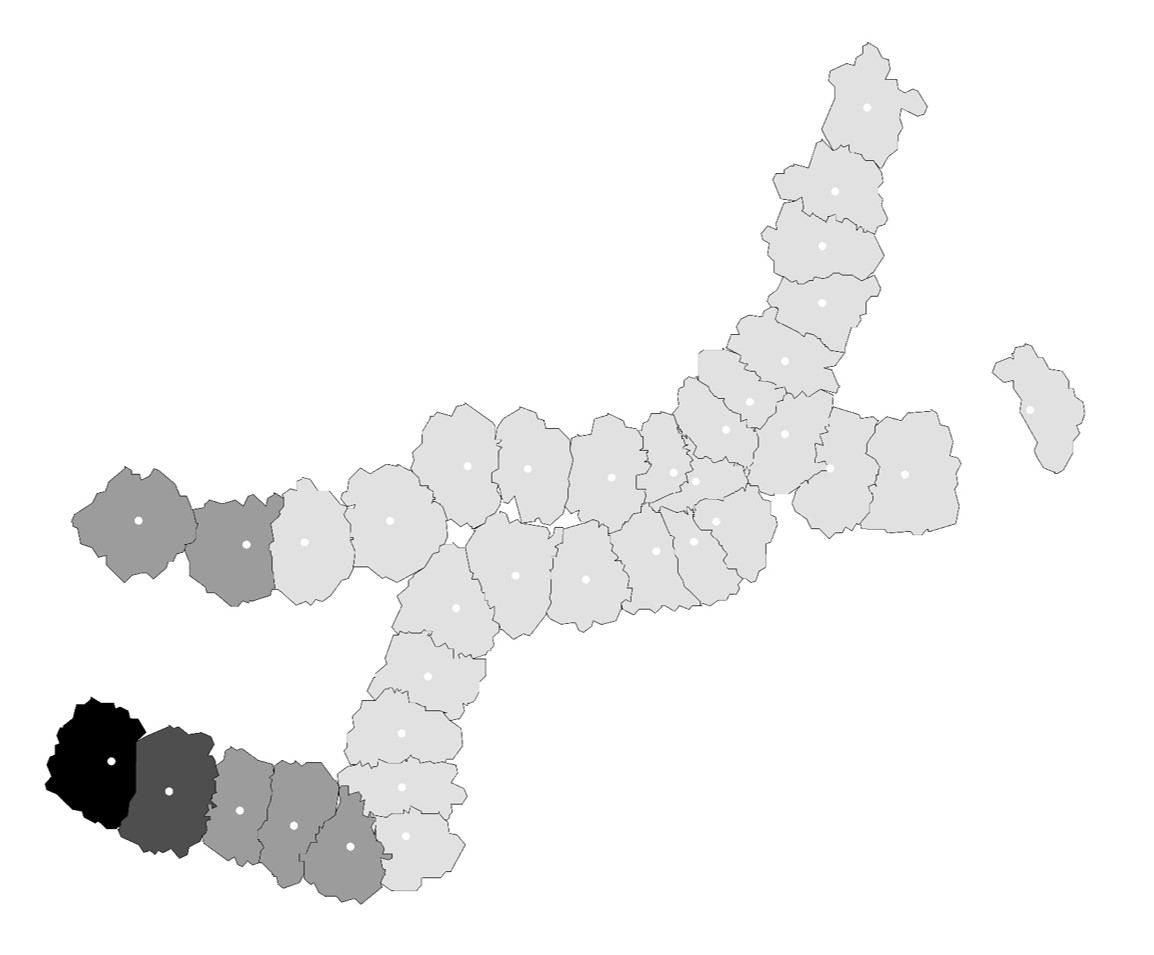
\includegraphics[width=\linewidth]{chp2TransportationFacility} % 这里的图片宽度是相对minipage的,所以1倍就可以了
		\centering{Transportation Facility}
	\end{minipage}
	\hfill % 横向填充,均匀分布
	\begin{minipage}{0.48\linewidth}
		\centering
		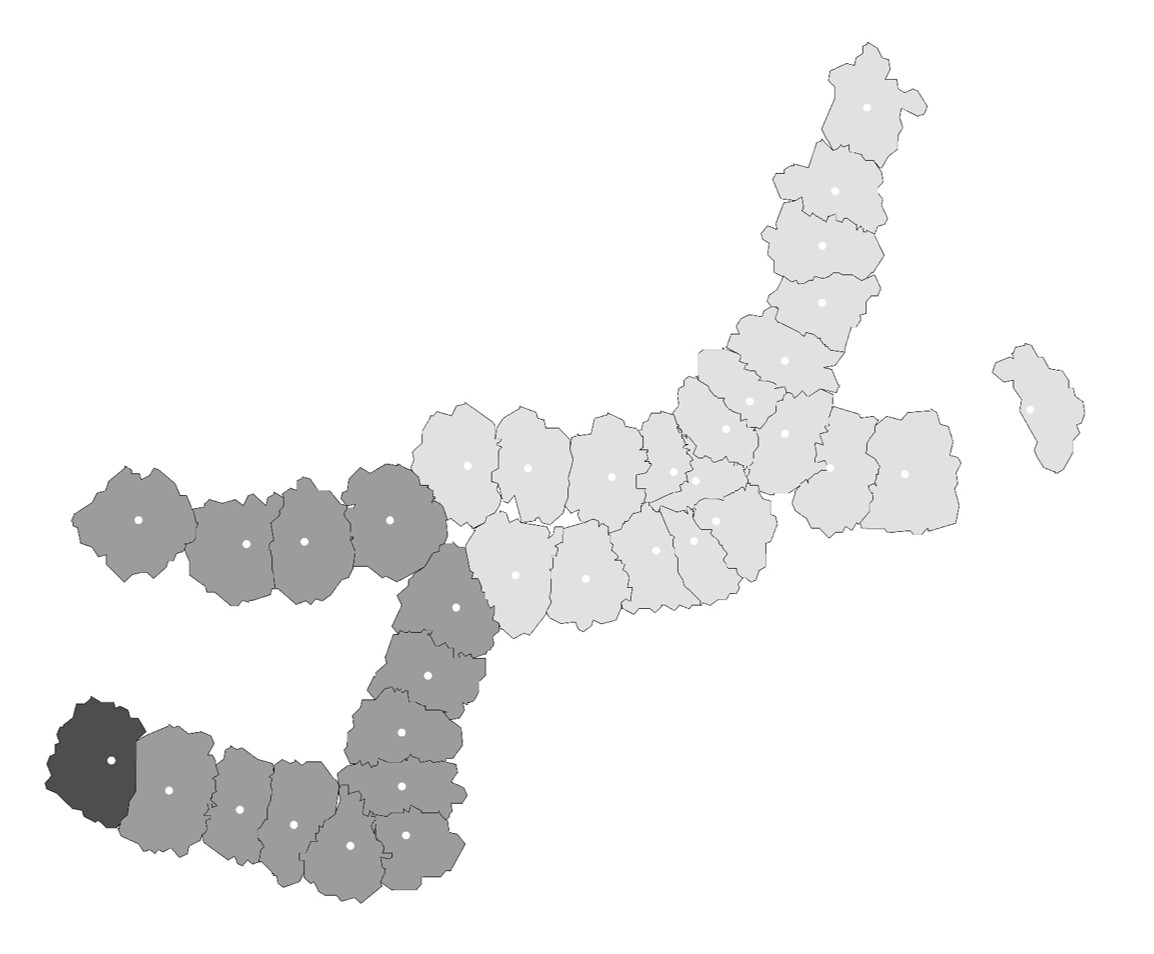
\includegraphics[width=\linewidth]{chp2BusCapacity}
		\centering{Bus Capacity}
	\end{minipage}
	
	\vfill % 纵向填充,均匀分布
	
	\begin{minipage}{0.48\linewidth}
		\centering
		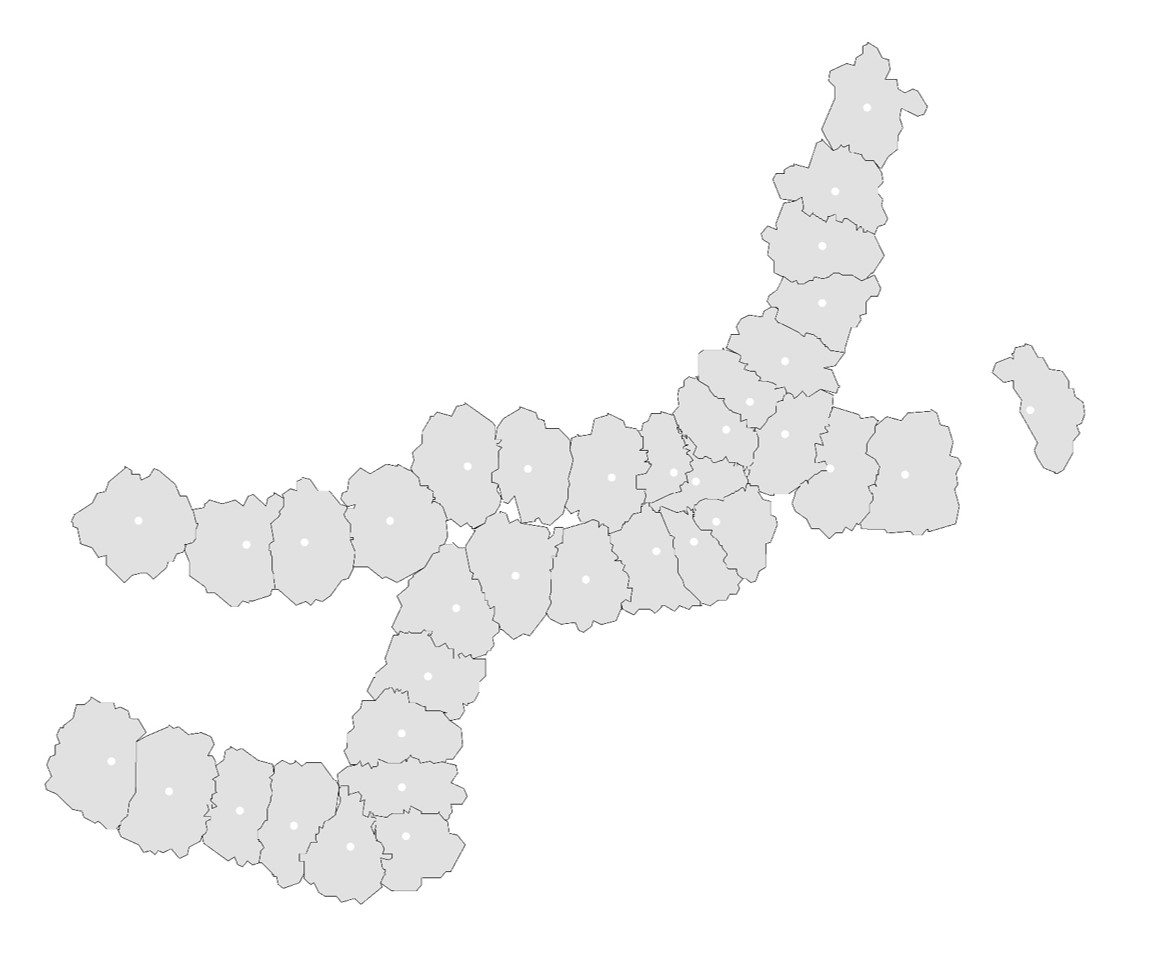
\includegraphics[width=\linewidth]{chp2BusAccessibility}
		\centering{Bus Accessibility}
	\end{minipage}
	\hfill
	\begin{minipage}{0.48\linewidth}
		\centering
		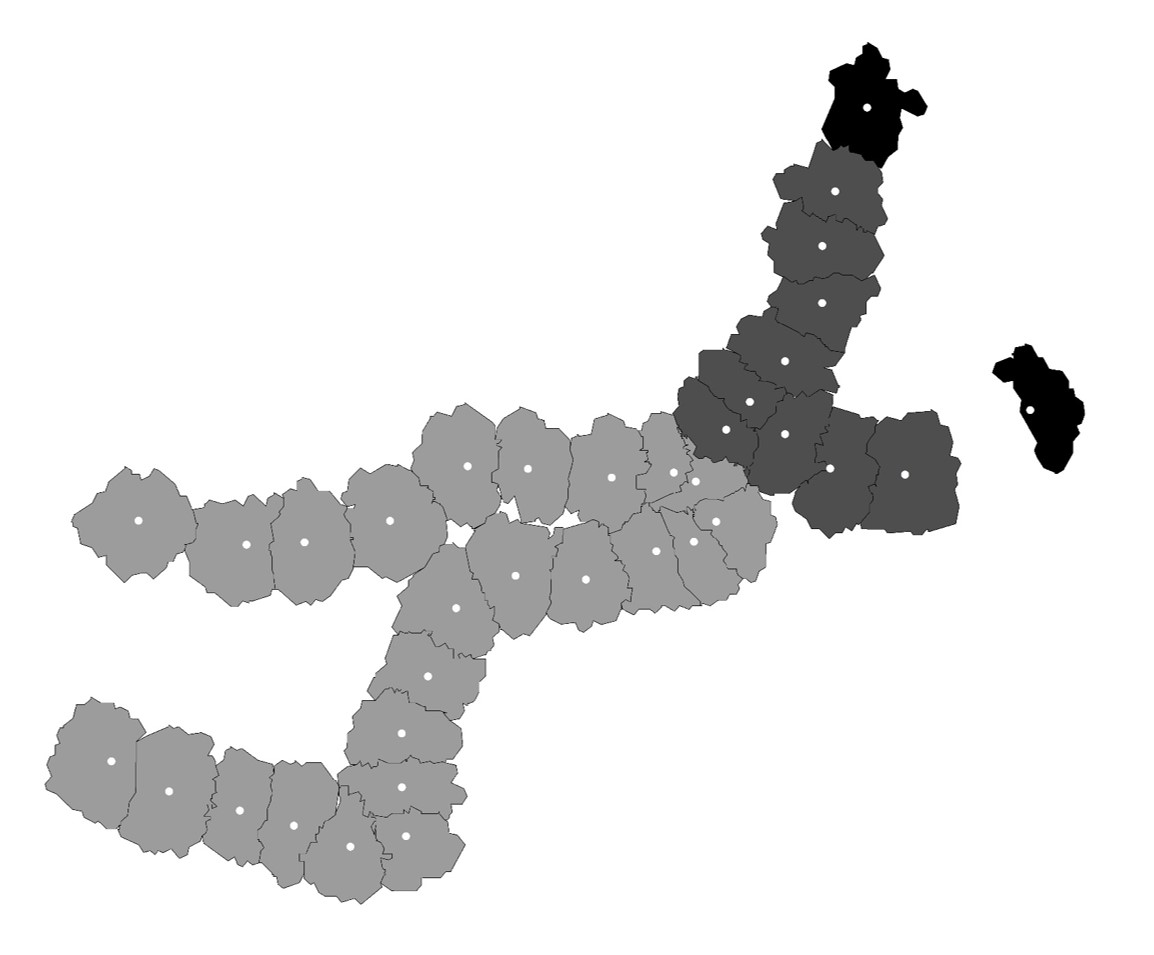
\includegraphics[width=\linewidth]{chp2PopulationJobBalance}
		\centering{Population Job Balance}
	\end{minipage}
	
	\vfill
	
	\begin{minipage}{0.48\linewidth}
		\centering
		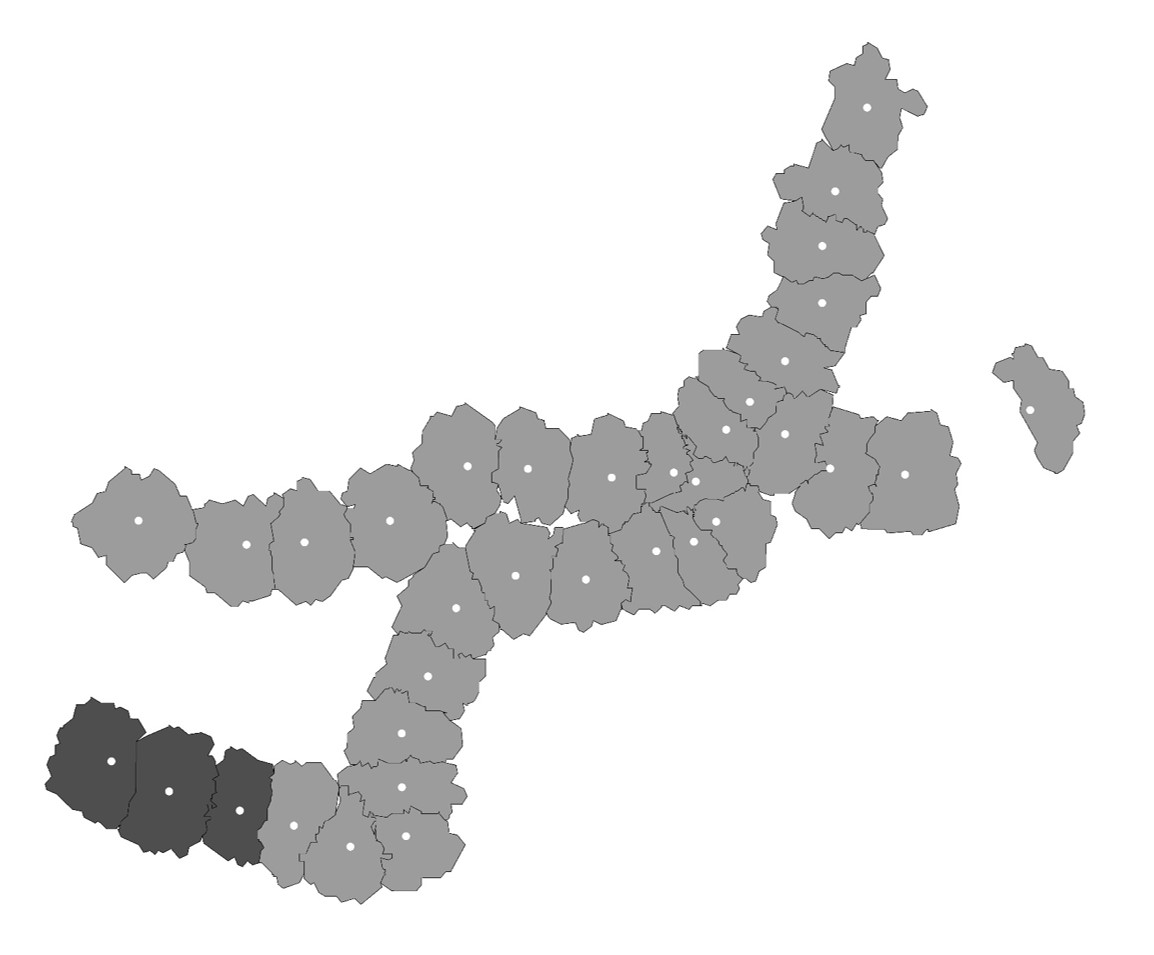
\includegraphics[width=\linewidth]{chp2TenantProportion}
		\centering{Tenant Proportion}
	\end{minipage}
	\hfill
	\begin{minipage}[c]{0.48\linewidth}
		\centering
		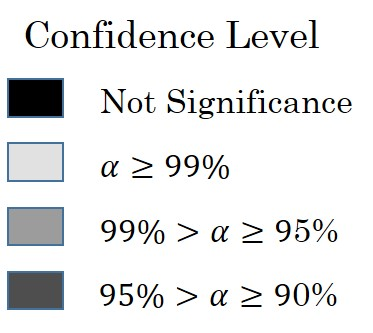
\includegraphics[scale=0.3]{chp2Legend}\\
	\end{minipage}
	
	\caption{The spatial distribution of significance level for local variables}
	\label{fig:chp2:SignificanceDistribution}
\end{figure}

%
\section{Discussion}
%
This study focuses on small sample size, using 9 explanatory variables to describe the variety of subway ridership in a local central city with 35 subway stations, while regarding the outcomes of some existed studies in Table \ref{tab:chp1:Review}, most of these studies have a middle sample size (ranged from 150-450), and the number of explanatory variables is general about 10. The adjusted $R^2$ (0.96) in this study is a relatively higher one comparing with other studies. Most of the variation in ridership can be explained by the 9 variables in this present model. But the adjusted $R^2$ is not the only judgment criterion in the regression model, especially in the small sample case. The result of this study shows that there are 3 variables, which are bus capacity, job-resident balance, and tenant proportion, impacting negative effect on ridership, while the others 6 variables plays positive effect. It is interesting to note from the coefficient that although the variables of bus capacity and bus accessibility have a strong positive correlation with statistical significance, they perform fully opposite effect on the independent variable. Regarding the coefficient showed in Table \ref{tab:chp2:ExploratoryRegression} and Table \ref{tab:chp2:ResultMGWR} obtained from the two models and 9 variables, the coefficients in both OLS model and MGWR model have consistent signs and similar values. The rationale of estimated results will be discussed from the three categories of indicators.

%
\subsection{Built environment}
%
Built environment has been considered as a critical driver for influencing transit ridership, and some results of empirical studies have supported it \cite{sohn2010factors,zhao2013influences,chakraborty2013land}. Built environment can reflect land use density around the station, different kind of building function has different demand in using subway \cite{chakraborty2013land}. In this study, two variables about building floor area (government area and transportation facility area) are found to be valid in explaining subway ridership (with statistical significance at 0.05 level). The coefficients showed in Table \ref{tab:chp2:ResultMGWR} implies that there is an increase of 5/10 passengers per additional 100 $m^2$ building floor area for government/transportation facility respectively. 

%
Refer to the results of previous studies, the building floor area of office and commerce was normally considered as the crucial driver for generating transit ridership. However, travel habit and culture are not the same in all cities. The result of this study stated that in Fukuoka people working at or visiting government office are likely to use the subway. Another valid indicator is building floor area of transportation facilities, which mainly represents the scale of public transit in the urban area. Obviously, the larger station usually has a larger scale of passengers, but the causal relationship is that forecasted ridership determined the scale of the station, rather than the opposite direction. Thus, this indicator of transportation facility can be viewed as an index for posterior evaluation, to judge if the planning is consistent with the fact, but not a predictable index. In fact, the variables of office area, commerce area, and residence area are also placed on the candidate list, but they are not showing statistical significance. One possible conjecture is given here: these three indicators represent the major category in building type, but they also contain several subcategories which cannot be expressed in the indicators. It means that each of these indicators is interpreting multiple issues, for which they cannot be consistent with statistics.

%
Moreover, the land use mix is also widely thought to be a crucial factor that can influence subway ridership. Some researches argued that the diversity of land use has a positive relationship with ridership, which means the higher diversity of land use can attract more passengers \cite{gutierrez2011transit,jun2015land}. However, the finding of this study shows an opposite result. The index of land use mix is redefined into land use aggregation in this study, and the result shows that the more aggregated the land use is the more ridership will be generated. In another word, the high diversity of land use will lead to a decrease in subway ridership. The relationship can be interpreted as following from the perspective of principles and features of TOD. A complete TOD area should have various kinds of urban function, and the main aim of TOD is to allow people to do their daily activities by walking in the TOD area, thus reducing inefficient vehicle trip. That is, if people can do most of their daily activities around the station, they will tend to reduce the use of subway. It is still not clear why this difference occurs. And unfortunately, the indicator of land use mix was not discussed in previous studies, there is little reference to explain it. A hypothesis is proposed to interpret this difference, even though there is no way to verify it, that is the proportion of each kind of land use should not be equal, the proportion in Fukuoka is as shown in Table \ref{tab:chp2:LandUse} \cite{bhat2007comprehensive}. Therefore, maybe this indicator with statistical significance in the prior studies was interpreting something else related to ridership but not describing land use mix. The results may be just statistically relevant to the ridership coincidentally. And that is the reason why this study proposes the method of identifying valid explanatory variables. Especially for small sample case, repeating test can reduce the probability of contingency.

%
\subsection{Transportation accessibility}
%
Accessibility is also thought to be a key factor influencing ridership. K. Sohn and H.Shim further divided this factor into internal and external accessibility, which was also cited and used by Zhao et al., the former represented the accessibility to station within the catchment area, and the latter reflected the connectivity to the place outside the catchment area \cite{sohn2010factors,zhao2013influences}. This study identified four valid variables in transportation accessibility: transfer dummy, bicycle parking, bus capacity and bus accessibility. The transfer dummy and bicycle parking can be easily classified into external accessibility and internal accessibility respectively, and both have a positive effect on ridership. It means the more easily people reach subway station, the more likely they will use the subway. This result is also consistent with prior studies \cite{gutierrez2011transit,cardozo2012application,kuby2004factors}.

%
However, the effect of bus service on subway ridership is not so intuitive and clear as other factors. It can be speculated that bus service may have both positive and negative effects on ridership, for there are both competitive and transferring relationships between bus and subway simultaneously. Therefore, a greater transport capacity of bus service can share part of the passengers of the subway while a more accessible route network, bus service can transfer more passengers to subway from other places. And the result from this study has verified this hypothesis that the indicator of bus accessibility and bus capacity showed the totally opposite effect on subway ridership, the former have a positive effect on subway ridership while the latter is in contrary. The indicator of bus service was intuitively considered to be related with subway ridership, and it often appears in the candidate variables list of prior studies, but is rarely estimated successfully in final model (some studies used the indicator of feeder bus rather than normal urban bus \cite{sohn2010factors,cardozo2012application,zhao2013influences}. Besides, the factor of trunk bus which is thought to be competitive with subway, is also considered in the previous study, but it did not show statistical significance \cite{sohn2010factors}. It can be guessed that the influence of bus service cannot be interpreted by only one indicator since the factor of bus service contains more than one kind of information. This result provided some inspiration that every transportation mode having both competitive and transferring relationships with another transportation mode may have both positive and negative effect on the others simultaneously.

%
\subsection{Demographic and social economic environment}
%
Regarding the factor of the demographic and socioeconomic environment, the job-resident balance and tenant proportion are found to be effective in explaining the variation of subway ridership. As shown in Table \ref{tab:chp2:ResultMGWR}, both job-resident balance and tenant proportion are showed to have a negative impact on subway ridership. The result indicates that working people tend to use subway more than unemployed people (like children, old people, and housewife), while tenant takes subway less.

%
Because the travel habit is not the same between working people and unemployed people, the indicator of job-resident balance is developed to help to interpret the difference between jobs and population. It is also suggested that job-resident balance is a crucial factor that can influence house price, this indicator is thought to be related to income level, family structure, social class an so on \cite{song2004measuring}. But whether and how it can influence subway ridership has not been verified yet in prior studies. The result from this study shows that job-resident balance can affect subway ridership, and it also can be inferred that different group of people has different travel habit. Moreover, the generally considered crucial indicator of population and employment is not showing validity in this study. One possible explanation is that these two variables have multicollinearity with other variables and they have been expressed in the combination of other variables.

%
In this study, tenant proportion is also verified that having a positive influence on subway ridership. But for different cities and regions, travel preferences are different. The result from the empirical case in nine US cities indicates that tenant is more likely to use subway, while the case in Seoul shows an opposite result that tenants living around station use subway less \cite{jun2015land,kuby2004factors}. It seems that renters are likely to use public transport, since they are thought to be poor, young, located in denser multifamily housing \cite{kuby2004factors}. However, the discussion also suggests that the indicator of tenant percentage should be treated separated: it may have a high tenant percentage in both CBD areas and suburban apartment, but of which the travel habits may be totally different. That means even though travel preference is different in CBD area and suburban area, the indicator of tenant proportion may be almost the same.

%
\subsection{Limitation and implication}
%
This study focuses on subway ridership at station level. However, the ridership of one station is not only influenced by the circumstance of itself but also the stations connected to it. Once the circumstance within catchment area changes, obviously, the ridership of this station will change as well. But the increased part of passengers will be transported to other stations, thus every station connected to that station will also have an increasing on ridership. Until now, most of the studies (including this study) on this issue are focusing on station level. Therefore, identifying and explaining the factors influencing subway ridership from both origin and destination will be the next step of research. Meanwhile, the analysis of subway ridership at station-to-station level based on OD data will also provide a way to research the spatial connectivity among the catchment area of subway stations.

\section{Conclusion}
%
This study examined the factors that may be associated with transit ridership using the case of subway stations in Fukuoka, Japan. There 9 effective factors selected from candidate indicators to describe the variation of subway ridership in the final models. The result from both the OLS and MGWR models shows that the 9 indicators performed stably and reasonable. The procedure proposed in this study is verified to be effective in identifying valid explanatory indicators in terms of small sample cases. The major contribution of this study can be summarized as follows.

%
First, on the base of previous studies, this study reclassified and reorganized the indicator framework. Besides the indicators appeared in the previous studies, the indicator of land use diversity was redefined as an aggregation of land use to make the expression of this index more intuitive and closer to reality. Additionally, two variables representing bus accessibility and bus capacity were proposed in this study to explore how can bus service influence the subway ridership.

%
Second, this study proposed an approach for identifying the valid indicators from all the candidate factors. The result shows that the valid indicators identified by this approach indeed has stable effect on the subway ridership of Fukuoka. In small sample cases, this approach is expected for it can reduce the probability of statistical error by repeating the trail regression.

%
Third, this study proposed an approach for distinguishing the global and local variables in MGWR model by using Moran’ Index. The result shows a significant improvement, even though in the case of a small sample, it performed reasonable and stable.

%
Finally, as a summary and prospect, direct station-level transit ridership forecasting model showed its advantages of rapid response, low cost, and high efficiency. But on the other hand, the direct model was still a part of the four step model, which could be viewed as the in-depth first step (forecasting of traffic generation) of the four step model. With the enrichment and diversification of data, the influence of environmental change in catchment area on transit ridership can be mastered more accurately with the help of GIS technology.

% reference
\clearpage % 新起一页
\bibliographystyle{apacite}
\bibliography{chapters/ref_AIJ}